\documentclass{article}

% Interpretiert die Folge von 0 und 1 als utf8 Encoding
% und erlaubt so Umlaute, Accents, Sonderzeichen, ...:
\usepackage[utf8]{inputenc}

\usepackage[T1]{fontenc}

% Abmessungen des Papiers, Ränder et cetera mit geometry.
% Hier erst mal nur Festlegung auf DIN A4 statt US letter Format.
\usepackage[a4paper]{geometry}


% Beide Packete für Mathe
\usepackage{amsmath}
\usepackage{amssymb}

% blindtext erzeugt Texte, die nur dazu dienen Platz im Dokument zu füllem.
% So sehen wir im Kurs wie sich Umbrüche verhalten et cetera.
\usepackage{blindtext}

\usepackage[english,ngerman]{babel}

\usepackage{graphicx}

\usepackage{float}

% Folgende Angaben werden nur in den Text eingefügt,
% wenn dort ein \maketitle zu finden ist!
\title{\LaTeX-Beispieldokument}
\author{\foreignlanguage{ngerman}{Rüdiger Voigt, M.A.}}
\date{\today}

\usepackage{hyperref}
\hypersetup{
hidelinks = true
}

\begin{document}

\maketitle

\begin{abstract}
\blindtext
\end{abstract}

% Inhaltsverzeichnis
\tableofcontents

% Abbildungsverzeichnis
\listoffigures

% Erzwinge Seitenumbruch
\newpage

% Mit \input können wir tex-Dateien über ihren Dateinamen 
% einbinden. Auf die Endung .tex kann dabei verzichtet werden.
\section{Einleitung}

\blindtext



\section{Text}

Eine Fußnote fügen Sie einfach mit dem Befehl \verb|\footnote{}| ein\footnote{So zum Beispiel}.\\
\\
Sie können mit \verb|\emph{}| \emph{Text hervorheben}.\\
\\
\textbf{Fettdruck} ist auch einfach.


\section{Floats}

\begin{figure}[htbp]
\centering
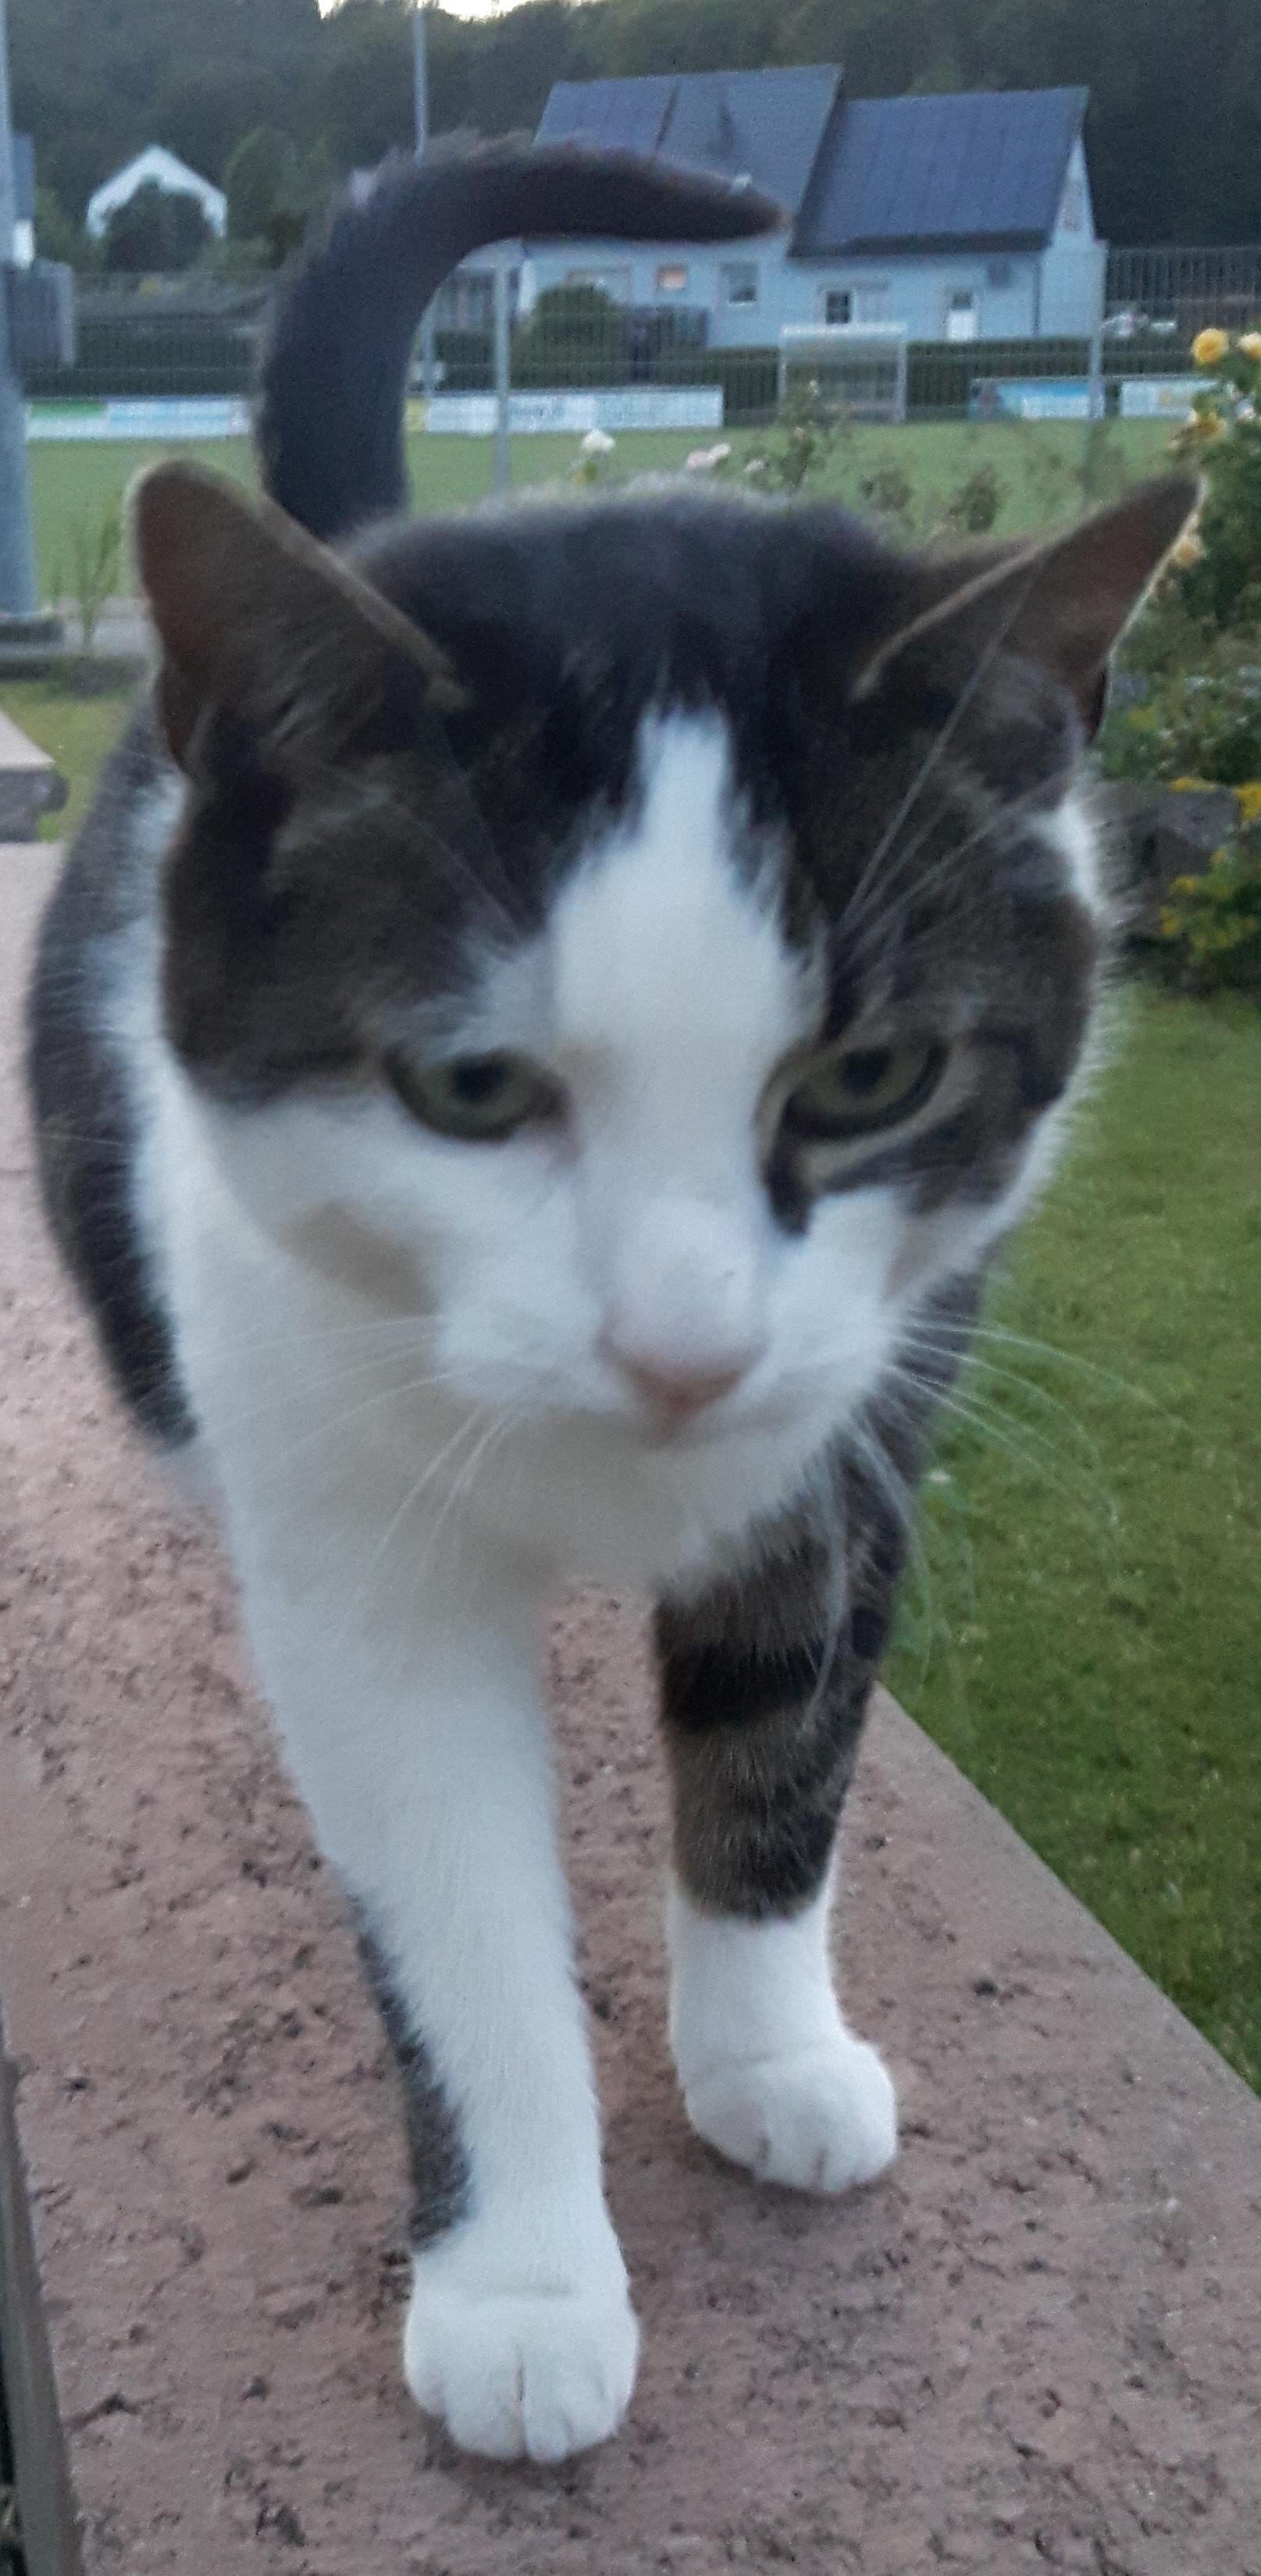
\includegraphics[width=0.5\textwidth]{img/2019-Dala-Mauer}
\label{img:cat}
\caption[Katze]{My cat in 2018}
\end{figure}

\section{Mathe}

Wenn Sie innerhalb des Fließtext mathematische Formeln einbinden möchten, umschließen Sie diese mit \$-Zeichen. Dann wird die Formel sehr kompakt dargestellt, wie zum Beispiel: $\sum_{i=1}^7$. Das macht nur Sinn für wenige komplexe Erläuterungen.
\\
Alternativ können Sie den abgesetzten Modus verwenden:

\[\sum_{i=1}^7\]


\noindent Die equation-Umgebung entspricht weitgehend dem abgesetzten Modus, aber fügt eine Nummerierung hinzu, die automatisch hochgezählt wird.

\begin{equation}
\sum = \pi \delta \$			
\end{equation}

\section{Abschnitt}

\Blindtext

\subsection{Referenzen}

Mit dem \verb|\ref{}| Befehl, können Sie ein vorher erstelltes Label referenzieren. Beispiel: Abbildung \ref{img:cat} auf Seite \pageref{img:cat}

\end{document}



















